\documentclass{beamer}
\setbeamertemplate{navigation symbols}{}
\usetheme{Malmoe}
\usecolortheme{beaver}
%\usepackage{natbib}   
%\bibliographystyle{plainnat}
\bibliographystyle{apalike}   % Or any other style you like
%\bibliographystyle{natbib} % kürzt automatisch vornamen ab und so zeug 
%\beamertemplatenavigationsymbolsempty
\beamersetuncovermixins{}{}
%\setbeamercovered{invisible}
%\usepackage{float}
\usepackage{amssymb}
\usepackage{wrapfig}
\usepackage{amsmath}
\usepackage[english]{babel}
\usepackage[utf8]{inputenc}
\usepackage{float}
\usepackage{graphicx}
%\usepackage{wrapfig}
\usepackage{textcomp}
\usepackage{braket}
\usepackage{bbm}
\usepackage{framed}
\usepackage{ifthen}
\usepackage{bbold}
\usepackage{colortbl}
\usepackage{xifthen}
\usepackage{color}
\usepackage{ifthen}
\usepackage[T1]{fontenc}
\usepackage{amsthm}
\usepackage{bm}
\usepackage{amsbsy}
\usepackage{tikz}
\usepackage{xspace}

\usepackage{xcolor}
\usepackage{scalefnt}
\usepackage{caption}
\addto\captionsngerman{
\renewcommand{\figurename}{Figure}%
\renewcommand{\tablename}{Tab.}%
}
\setlength{\parskip}{1.5ex plus0.5ex minus0.5ex}
\setlength{\parindent}{0em} 

\sloppy \frenchspacing \raggedbottom 


\usetikzlibrary{trees}
\usetikzlibrary{positioning}
\tikzset{main node/.style={circle,fill=black,draw,minimum size=3pt,inner sep=0pt},}
\tikzset{
    invisible/.style={opacity=0,text opacity=0},
    visible on/.style={alt=#1{}{invisible}},
    alt/.code args={<#1>#2#3}{%
      \alt<#1>{\pgfkeysalso{#2}}{\pgfkeysalso{#3}} 
    },
    beameralert/.style={alt={<#1>{fill=red!30,rounded corners}{}},anchor=base},
    BeamerAlert/.style={alt={#1{fill=red!30,rounded corners}{}},anchor=base}
}
  \newcommand<>{\tikzMe}[1]{% previously: \def\tikzMe<#1>#2{…
    \tikz[baseline]\node[BeamerAlert={#2},anchor=base] {#1};
}

%\usetikzlibrary{external}
%\tikzexternalize[prefix=external]
\usepackage{verbatim}

\newcommand{\V}{\ensuremath{\mathbf{V}}\xspace}
\newcommand{\F}{\ensuremath{\mathbf{F}}\xspace}

% Prov makro
\DeclareMathOperator*{\Prov}{Prov}
\DeclareMathOperator*{\Var}{Var}

\DeclareMathOperator*{\Proov}{Proof}

\newcommand{\NP}{\ensuremath{\mathcal{NP}}}
\begin{document}
\title{Formula Evaluation}
\author{Abraham Hinteregger}
\institute{Vienna University of Technology}
\date{2016-06-07}
\titlepage
\setcounter{tocdepth}{3}
\AtBeginSection[]{
\begin{frame}
\frametitle{Chapter} 
\tableofcontents[currentsection,currentsubsection,hideothersubsections]
\end{frame}
}


\section{Logic as a game}
\setbeamertemplate{footline}[frame number]

\begin{frame}{Motivation}
\begin{itemize}
\item Given is a formula $\varphi$ in a model $M$ with a variable setting $s$ 
\item In model-theoretic semantics the question was whether this formula is true in this model with the setting ($M,s \models \varphi$) or not ($M,s\nvDash\varphi$)
\item If one person thinks the formula is true and another person doubts that an obvious game arises:
\begin{itemize}
\item The first person (verifier, \V) tries to verify that the formula is true 
\item the second person (falsifier, \F) tries to do the opposite
\end{itemize}
\end{itemize}
\end{frame}

\subsection{Predicate logic}
\begin{frame}\frametitle{First order predicate logic (reminder\footnote{in the spirit of CI})}
\begin{itemize}
\item A formula is built from formulas ($A, B,\ldots$) and operators:
\begin{itemize}
\item Constants $\top,\bot$
\item  Unary negation operator $\lnot A$
\item Binary operators $\land, \lor$: $A \circ B$
\item Quantifiers $\exists, \forall$: $\exists xA(x), \forall x B(x)$
\item Predicates, e.g. $A(x), B(x,y)$
\end{itemize}
\item A model is a set of objects, also called the universe/domain 
\begin{itemize}
\item Constants are mapped to an object in the domain
\item Functions map one (or more) objects in the domain to another object in the domain
\item Predicates are mapped to a subset of the domain 
\end{itemize}
\end{itemize}
\end{frame}

\begin{frame}\frametitle{Evaluation games for predicate logic} 
\begin{tabular}{ll}
atoms  $P(x), R(x,y),\top,\bot$ &  \V wins if atom is true, else \F wins\\
disjunction $\varphi \lor \psi$ & \V chooses which disjunct to play\\
conjunction   $\varphi \land \psi$ & \F chooses which conjunct to play\\
negation  $ \lnot \varphi$ & role switch of the two players\\\\\hline\\
existential quantifier $\exists x\varphi(x)$ & \V  picks an object $d$ from the domain\\
universal quantifier $\forall x \varphi(x)$& \F picks an object $d$ from the domain
\end{tabular}
\end{frame}


\subsection{Modal logic}
\begin{frame}{Evaluation games for modal logic}
\begin{itemize}
\item Rules from evaluation games for predicate logic
\item Additional rules that accomodate for the modal operators $\Box$ and $\Diamond$ (or indexed versions $\Box_i, \Diamond_i$):
\begin{tabular}{ll}\\
necessity $\Box P$ & \F chooses a successor of the current world\\
possibility $\Diamond P$ & \V chooses a successor of the current world\\\\
\end{tabular}
Failure to choose a successor means a loss for either player
\item Game state consists not only of setting $s$ and current formula $\varphi$ but also the current world $w$.

\end{itemize}
\end{frame}


%\subsection{Examples}
\begin{frame}\frametitle{Example of evaluation games for predicate logic} 
    {
\uncover<2->{(domain consists of two objects, $s$ and $t$)}
\begin{tikzpicture}[grow=down, sloped]
% Set the overall layout of the tree
\tikzstyle{level 1}=[level distance=2.5cm, sibling distance=6cm]
\tikzstyle{level 2}=[level distance=2.5cm, sibling distance=3cm]

% Define styles for bags and leafs
\tikzstyle{bag} = [text width=4em, text centered]
\tikzstyle{end} = [circle, minimum width=3pt,fill, inner sep=0pt]
\uncover<2>{

\node[bag] {\F\\ ${\forall x \exists y\ x\neq y}$}
    child[opacity=0] {
	node[bag] {\V\\$\exists y s \neq y$}        
		child {
			node[end, label=right:{$lose_V; s\neq s$}] {}
			edge from parent node[above] {$y:=s$}
		}
		child {
			node[end, label=right:{$win_\V; s\neq t$}] {}
			edge from parent node[above] {$y:=t$}
		}
	edge from parent node[above] {x:=s}
    }
    child[opacity=0] {
        node[bag] {\V\\${\exists y t\neq y}$}        
        child {
                node[end, label=right:{$win_\V; s\neq t$}] {}
                edge from parent node[above] {$y:=s$}
            }
            child {
                node[end, label=right:{$lose_\V; t\neq t$}] {}
                edge from parent node[above] {$y:=t$}
            }
        edge from parent         
            node[above] {$x:=t$}
    };}
\uncover<3>{

\node[bag] {\F\\ ${\forall x \exists y\ x\neq y}$}
    child {
	node[bag] {\V\\$\exists y\ s \neq y$}        
		child[opacity=0] {
			node[end, label=right:{$lose_V; s\neq s$}] {}
			edge from parent node[above] {$y:=s$}
		}
		child[opacity=0] {
			node[end, label=right:{$win_\V; s\neq t$}] {}
			edge from parent node[above] {$y:=t$}
		}
	edge from parent node[above] {x:=s}
    }
    child {
        node[bag] {\V\\${\exists y\ t\neq y}$}        
        child[opacity=0] {
                node[end, label=right:{$win_\V; s\neq t$}] {}
                edge from parent node[above] {$y:=s$}
            }
            child[opacity=0] {
                node[end, label=right:{$lose_\V; t\neq t$}] {}
                edge from parent node[above] {$y:=t$}
            }
        edge from parent         
            node[above] {$x:=t$}
    };}
\uncover<4>{

\node[bag] {\F\\ ${\forall x \exists y\ x\neq y}$}
    child {
	node[bag] {\V\\$\exists y\ s \neq y$}        
		child {
			node[bag, label=below:{$lose_\V$}] {$s\neq s$}
			edge from parent node[above] {$y:=s$}
		}
		child {
			node[bag, label=below:{$win_\V$}] {$s\neq t$}
			edge from parent node[above] {$y:=t$}
		}
	edge from parent node[above] {x:=s}
    }
    child {
        node[bag] {\V\\${\exists y\ t\neq y}$}        
        child {
                node[bag, label=below:{$win_\V$}] {$t\neq s$}
                edge from parent node[above] {$y:=s$}
            }
            child {
                node[bag, label=below:{$lose_\V$}] {$t\neq t$}
                edge from parent node[above] {$y:=t$}
            }
        edge from parent         
            node[above] {$x:=t$}
    };}
\end{tikzpicture}
}
\end{frame}


%\subsection{Examples}
\begin{frame}\frametitle{Example of evaluation game for modal logic} 



 \begin{columns}[T]
    \begin{column}{.5\textwidth} {
    
\begin{itemize}
\item If \V chooses world $3$ \F can't move and loses
\item Else \V  can choose either world 1 or 2 and wins no matter what \F does
\end{itemize}   

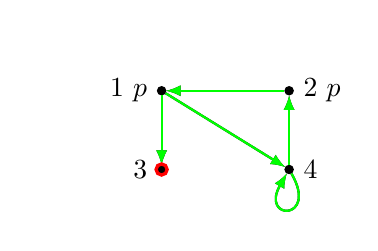
\begin{tikzpicture}[grow=down, sloped]

 \node[main node,label=left:{1 $p$}] (1) {};
    \node[main node,label=left:{3}] (3) [below of = 1]  {};
    \node[main node,label=right:{2 $p$}] (2) [right = 1.5cm of 1] {};
    \node[main node,label=right:{4}] (4) [below of = 2] {};
     \path[-latex,draw,thick]    (2) edge node {} (1);
     \path[-latex,draw,thick]    (1) edge node {} (3);
     \path[-latex,draw,thick]    (4) edge node {} (2);
     \path[-latex,draw,thick]    (1) edge node {} (4);
     \path[-latex,draw,thick]    (4) edge [out=300,in=240,looseness=30] node {}(4);


\uncover<1>{
%	\draw[green, very thick](1) circle(2pt);
	\path[green,  thick, -latex, draw](1) edge node{} (4);
	\path[green,  thick, -latex, draw](1) edge node{} (3);
};

\uncover<2>{
	\draw[red, very thick](3) circle(2pt);
};

\uncover<3-4>{
%	\draw[green, very thick](4) circle(2pt);
	\path[green,  thick, -latex, draw](4) edge[out=300,in=240,looseness=30] node{} (4);
	\path[green,  thick, -latex, draw](4) edge node{} (2);
};

\uncover<5>{
%	\draw[green, very thick](2) circle(2pt);
	\path[green,  thick, -latex, draw](2) edge node{} (1);
};



%ugly hacks follow
\node[opacity=0](y) [above = 0.5cm of 1]{}; % some spacing above 
\node[opacity=0](x) [left = 1.4cm of 1]{}; % for centering
\end{tikzpicture}
}
\end{column}
 
    \begin{column}{.5\textwidth}
  %  \begin{block}
  {
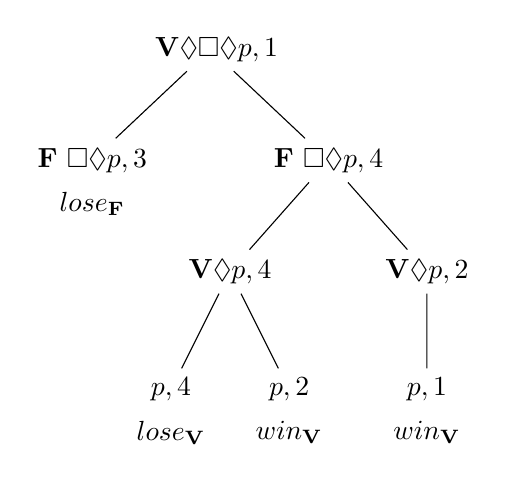
\begin{tikzpicture}[grow=down, sloped]
% Set the overall layout of the tree
\tikzstyle{level 1}=[level distance=1.5cm, sibling distance=3cm]
\tikzstyle{level 2}=[level distance=1.5cm, sibling distance=2.5cm]
\tikzstyle{level 3}=[level distance=1.5cm, sibling distance=1.5cm]
% Define styles for bags and leafs
\tikzstyle{bag} = [text width=4em, text centered]
\tikzstyle{end} = [circle, minimum width=3pt,fill, inner sep=0pt]



\node[beameralert=1,bag] { ${\V\Diamond\Box\Diamond p,1}\quad $}
    child {node[beameralert=2,bag,label=below:{$lose_\F$}] {\F $\Box\Diamond p, 3$}}
    child {node[beameralert=3,bag] { ${\F\ \Box\Diamond p, 4}$}        
	child {node[beameralert=4,bag] {{$\V \Diamond p, 4$}}
		child {node[bag, label=below:{$lose_\V$}] {$p, 4$}}
		child {node[bag, label=below:{$win_\V$}] {$p, 2$}}
	}
	child {node[beameralert=5,bag] {$\V \Diamond p, 2$}
		child {node[bag, label=below:{$win_\V$}] {$p, 1 $}}
          }
   };

\end{tikzpicture}
}
    %\end{block}
    \end{column}
 
\end{columns}
\end{frame}




\begin{frame}
\frametitle{Some observations}
\begin{itemize}[<+->]
\item Both players can choose between two options (assigning either $s$ or $t$ to $x,y$ or deciding a successor for the current world)
\item Both players can win and lose but only \V does influence the outcome of the games (\F cannot even force a loss)
\item \V has a winning strategy (``don't assign the same thing as \F'', ``go to world 1 or 2'')
\item In the second game \V has even two strategies for winning (``pick 3'', ``pick 4 and then pick either 2 or 1'')
\end{itemize}
\end{frame}

%\section{Properties}
\subsection{Determinacy}
\begin{frame}{Determinacy\footnote{Hintikka referred to this as ``determinateness'' \cite{hintikka}}}
%Player A has a winning strategy if he can react to any move the opponent plays with at least one move s.t. A wins the game
\begin{block}{Success Lemma}
$M,s\models \varphi \Longleftrightarrow \text{\V has a winning strategy in $game(\varphi,M,s)$}$\\
$M,s\not\models \varphi \Longleftrightarrow \text{\F has a winning strategy in $game(\varphi,M,s)$}$

Proof by induction on formulas:
\begin{itemize}
%\item For atoms it obviously holds
\item If $v_M(\varphi \lor \psi) = 1 $: w.l.o.g. $v_{M}(\varphi) = 1$. By inductive hypothesis \V has a winning strategy for $game(M,s,\varphi)$ and thus also for $game(M,s,\varphi\lor\psi)$
\item If $v_M(\lnot \varphi) = 1$: $\implies v_M(\varphi) = 0$ and by IH \F has a winning strategy for $game(M,s,\varphi)$. Player switch yields a winning strategy for \V for $game(M,s,\lnot \varphi)$.
\item \ldots
\end{itemize}
\end{block}
\end{frame}

\begin{frame}{Determinacy II}
\begin{itemize}
\item Complexity of formula strictly decreases as game continues until only atomic formula is left
\item At every branching the active player has a winning strategy if there is a winning strategy available for at least one of the branches
\item As this propagates to the root there's a winning strategy for at least (and at most) one of the two players.
\item This theory of truth coincides with Tarski's truth definition
\end{itemize}
\end{frame}

%\begin{frame}{Determinacy III}
%\begin{itemize}
%\item<1-> Truth in model theoretic semantics corresponds 1:1 to existence of winning strategy for either player
%\item<2-> Great\ldots \uncover<3->{ but rather unexciting}
%\item<3-> Is it possible to extend this?
%\begin{itemize}
%\item<4-> One winning strategy versus more of them
%\item<4-> Losing intentionally
%\end{itemize}
%\end{itemize}
%\end{frame}


\section{Game view of logic \& extensions}
\subsection{Formal definition of the game}
\begin{frame}{Inductive definition of the game}
A game ``$game(M,s,\varphi)$'' is defined as a tree where every node is a pair $(s,\psi)$ where $s$ is an $M$-assignment and $\psi$ is a subformula of $\varphi$.\\
\begin{tabular}{c| l}\hline
$\varphi$ & Interpretation of $game(M,s,\varphi)$\\\hline
atomic & one node game where \V wins iff $M,s\models\varphi$\\
$\exists x$ &game where \V picks any available move $s[x:=d]$ and wins
\\\\
$\phi \lor \psi$ & game is disjoint union of two games and it's \V's turn\\
$\phi \land \psi$ & same as above but it's \F's turn\\
$\lnot \phi$ & $game(M,s,\phi)$ with win markings reversed\\\\
$\phi; \psi$ & Game arising by taking $game(M,s,\phi)$ with assignment $t$ \\&at end states and continuing with $game(M,t,\psi)$
\end{tabular}
\end{frame}

\begin{frame}{Extended syntax of formulas}
The changed quantifier and composition rules allow formulas such as:
\begin{itemize}[<+->]
\item $\exists x$: \V chooses new assignment $s[x:=d]$ and wins.
\item $P(x); \exists x$: Test whether $P(s(x))$ holds and then assign a new value to $x$. 
\end{itemize}
\end{frame}

\subsection{Additional moves}
\begin{frame}{Additional moves\footnote{Chapter 16, \cite{lig}}}
Until now the model $M$ was fixed and remained unchanged. The game could be extended by allowing moves that manipulate the model in some way:
\begin{itemize}
\item Adding or removing objects from the domain
\item Changing the interpretation
\end{itemize}
\end{frame}

\subsection{More refined semantics}
\begin{frame}{Refined semantics\footnote{Chapter 15, \cite{lig}}}
\begin{itemize}
\item Difference between the existence of one winning strategy and many of them. 
\item How many moves does a strategy need to win?
\item Is it possible to lose on purpose?
\end{itemize}
\end{frame}




%\begin{frame}
%\cite{sep-logic-games}
%\cite{sep-logic-dialogical}
%\cite{lig}
%\cite{insightshintikka}
%\end{frame}


\section{Stuff}
\subsection{References}
\begin{frame}[allowframebreaks]{References}
\nocite{*} %load everything from log.bib
\bibliography{log}
\end{frame}


\subsection{Modal $\mu$-calculus}
\begin{frame}\frametitle{Modal $\mu$-calculus\footnote{\cite{venema}}}
Adds two additional operators to propositional (multi-) modal logic:
\begin{itemize}
\item Least fixpoint operator $\mu p: \varphi(p)$ 
\item Greatest fixpoint operator $\nu p: \varphi(p)$
\end{itemize}
Note that $p$ occurs positively in $\varphi(p)$, meaning that there's an even amount of $\lnot$ in front of every occurence of $p$ in $\varphi$\footnote{The positive syntactic occurence of $p$ implies monotonicity concerning inclusion $\implies$ least and greatest fixpoint exist \cite{knaster}.}
\end{frame}

\begin{frame}{Examples for modal $\mu$-calculus}
\begin{tabular}{l l}
Formula & Interpretation\\\hline
\uncover<+->{$\mu p : (q \lor \Diamond p)$ & \uncover<+->{Set of all worlds $w$ where a world $v$ s.t. $M,v\models q$ \\&is reachable with \alert<7>{finite} path}} \\\\
\uncover<+->{$\nu p : (q \land \Box_a p)$ & \uncover<+->{Set of all worlds $w$ where $M,w\models q$ on \alert<7>{every} $a$-path}}\\\\
\uncover<+->{$\nu p : (\Diamond \top \land \Box p)$ & \uncover<+->{Set of all worlds that have outgoing transitions\\& and don't have a path to a world without\\& outgoing transitions}}\\\\
\end{tabular}
\uncover<8->{$\nu$ means unfolding, $\mu$ means finite unfolding}
\end{frame}


\subsection{Evaluation game for $\mu$-calculus}
\begin{frame}{Evaluation game for $\mu$-calculus}
\begin{itemize}
\item Rules from modal evaluation game
\item If fixed point formula $\mu p : \varphi(p)$ or $\nu p : \varphi(p)$ is reached, the game proceeds with $\varphi(p)$
\item<2-> $p$ is not an atom but a bound variable and instead of testing the atom the original fixed point formula is substituted back in. 
\item<3-> If the evaluation loops (node visited multiple times) \V wins if the infinitely many times substituted variable is bound to a $\nu$- formula and \F wins if it's bound to a $\mu$- formula\footnote{if there is more than one such variable the one with highest rank (contains the others as subformulas) counts}
\end{itemize}
\end{frame}



\end{document}
